\chapter{Familiarizing Yourself with Simulink}\label{Lab:1}
Low-pass filters are ubiquitous. They can be found in the hardware of
audio processing chips, or the software of image editing tools. As you may
recall from a course on Signals and Systems theory\footnote{If you haven't
taken a course in Signals and Systems, speak to your Lab Instructor on
knowledge you may be lacking.}, a low-pass filter
is a system that, generally speaking, rejects high-frequency signals while
``passing through'' low-frequency signals. In this lab you will be asked
to analyze a low-pass filter block and determine its parameters via a time
domain approach. This is not meant to be a difficult lab and is instead
designed to give you a sense of the lab format.

\section{Objectives}
The primary objectives of this lab are to
\begin{enumerate}[label=(\arabic*)]
  \item{
    Install MATLAB, Simulink and required toolboxes.
    Alternatively, connect remotely to
    \url{engterm.uwaterloo.ca} or any other lab computer of your choice
    that has MATLAB.
  }
  \item{
    Understand how to create a Simulink diagram and how to run
    a simulation.
  }
  \item{
    Understand how to log signals for future inspection and how to then
    make time-domain measurements.
  }
\end{enumerate}
The list of required deliverables is not very large so you should
spend your time exploring Simulink so as to reduce the amount of time
you spend on future labs. That is, of course, not a requirement but I recommend
you do so.

\section{Experimental Procedure}
This entire lab will be done using the ``\texttt{Lab\_1.slx}'' Simulink model.
In there you will
find five blocks already placed for you in an open loop configuration:
\begin{itemize}
  \item{a signal generator,}
  \item{a summing junction,}
  \item{an adjustable gain block,}
  \item{a ``plant'', the system we are going to analyze, and}
  \item{a terminator.}
\end{itemize}
You do not require any more blocks than these. You will be asked to add
a new path.

\subsection{Acquiring the Bandwidth in Time-Domain}
The goal of this portion of the lab is to acquire the bandwidth of the
given linear system. What is the bandwidth? To understand and acquire it,
we must first know what the DC gain of a system is.
%
\begin{definition}[DC Gain]
  Let \(G(s)\) be a \emph{stable} transfer function
  that maps an input signal \(U(s)\) to an
  output \(Y(s).\) The \textbf{DC gain} of \(G(s)\) is \(G(0)\) and,
  if \(u(t) = A \mathbf{1}(t)\) for \(A \in \Real,\) it satisfies the relation
  \[
    \lim_{t\to \infty} y(t) = A G(0).
  \]
\end{definition}
%
Observe that the DC gain \(G(0)\) is called precisely that because when we
apply a square (DC-like; step) signal change, the system's output converges
to the amplitude of the input times \(G(0).\)
%
Instead of computing the DC gain by evaluating the system's response to a step
input, we take a different approach.
%
\begin{procedure}
  You will acquire the DC gain of the plant \(P(s)\). Follow these steps:
  \begin{enumerate}[label=(\arabic*)]
    \item{
      \textbf{Open} the signal generator block, and set the
      \textbf{amplitude} to be \(1\) and the \textbf{frequency}
      to be \(\SI{0.5}{Hz}.\) This signal is so low frequency that it
      emulates a constant signal.
    }
    \item{
      \textbf{Run} the script \texttt{generate\_lab\_1\_plot.m} and inspect
      Figure 1, which depicts the input and output signal.
    }
    \item{
      \textbf{Measure the amplitudes} of the input and output signals
      respectively when the system is in steady-state. In simulation, this
      amounts to performing this measurement near the end of the simulation
      time.
    }
    \item{
      \textbf{Estimate} the DC gain by dividing the output amplitude
      by the input amplitude. \emph{Remember, we chose the input amplitude
      to be \(1\)!}
    }
  \end{enumerate}
  \label{lab1:p1}
\end{procedure}
%
\begin{figure}
  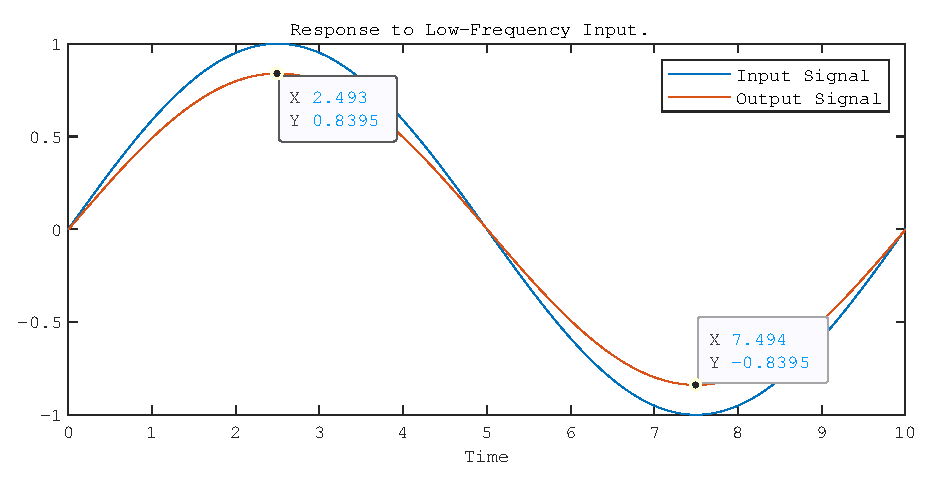
\includegraphics{images/Lab_1_LowFrequency.eps}
  \caption{The low-frequency response to my low-pass plant \(P(s).\) The gain
  at this low frequency is \(0.8395.\) Can you see why? What is the DC
  gain approximately?}
  \label{fig:lab1:lowfreq}
\end{figure}
%
\begin{deliverable}
  \textbf{Record} your estimated DC gain and \textbf{capture} the generated
  figure with the cursors you used to measure the amplitudes.
  Your figure should like Figure~\ref{fig:lab1:lowfreq}.
  \label{lab1:d1}
\end{deliverable}
%
For low-pass systems, as we increase the frequency of the input, we will
observe, the output amplitude \emph{decreases}. The bandwidth frequency
is the frequency that marks the point where we distinguish between the
``low'' frequency inputs a low-pass system sustains and the ``high'' frequency
inputs a low-pass system rejects.
%
\begin{definition}[Bandwidth]
  Let \(G(s)\) be a proper transfer function
  that maps an input signal \(U(s)\) to an output \(Y(s).\)
%
  Say the input is a sinusoid of the form \(A \cos(\omega t)\) with amplitude
  \(A.\) In steady-state, the amplitude of \(y(t)\) converges to a constant
  \(B.\) The \textbf{gain at frequency \(\omega\)} is
  \(\left\|G(j\omega)\right\| = \frac{B}{A}.\)
%
  The \textbf{bandwidth (frequency)} of \(G(s)\) is the \emph{smallest}
  frequency \(\omega\) which satisfies
  \[
    \frac{1}{\sqrt{2}} = \frac{\left\|G(j\omega)\right\|}{\left\|G(0)\right\|}.
  \]
\end{definition}
%
Simply put, the bandwidth frequency is where we find the gain has
dropped by a factor of \(\sqrt{2}\) in comparison to the DC gain.
Figure~ depicts this. We can see when we apply
%
\begin{procedure}
  You will acquire the bandwidth frequency of the plant \(P(s)\).
  Follow these steps:
  \begin{enumerate}[label=(\arabic*)]
    \item{
      \textbf{Predict} the amplitude of the steady-state output at the
      bandwidth frequency. As an example, if your DC gain is \(0.8395\) then
      the ratio between the input signal amplitude and the output signal
      at the bandwidth frequency is
      \[
        \frac{0.8395}{\sqrt{2}}.
      \]
      If my input signal has amplitude \(1,\) then I should look for
      an output signal amplitude with the above value.
    }
    \item{
      \textbf{Open} the signal generator block, and set the
      \textbf{amplitude} to be \(1\) and
      the \textbf{frequency} to be \(\SI{0.5}{Hz}.\)
      \label{lab1:p2:2}
    }
    \item{
      \textbf{Run} the script \texttt{generate\_lab\_1\_plot.m} and inspect
      Figure 1, which depicts the input and output signal.
    }
    \item{
      \textbf{Measure the amplitudes} of the output signal
      when the system is in steady-state.
      \label{lab1:p2:4}
    }
    \item{
      If the amplitude isn't what you want, repeat Steps~\ref{lab1:p2:2} through~\ref{lab1:p2:4} with a different frequency. Increase or decrease
      by orders of magnitude to speed up the process!
    }
    \item{
      If the amplitude is what you predicted, \textbf{record} the frequency
      of the input you used to achieve the result.
    }
  \end{enumerate}
  \label{lab1:p2}
\end{procedure}
%
\begin{figure}
  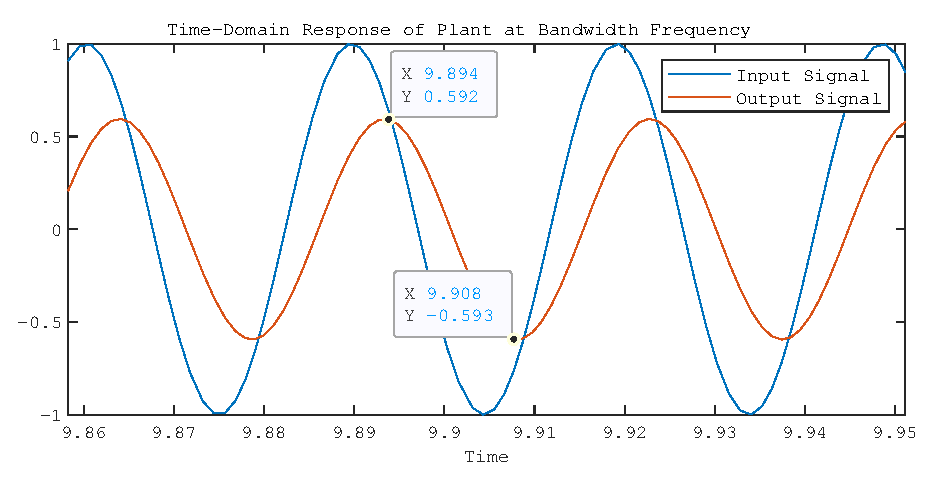
\includegraphics{images/Lab_1_Bandwidth.eps}
  \caption{The response to my \(P(s)\) at the bandwidth frequency.
  Can you see why this is the bandwidth frequency for my plant?}
  \label{fig:lab1:bandwidth}
\end{figure}
%
\begin{deliverable}
  At the bandwidth frequency,
  \textbf{capture a figure} of the input and output signal. It should look
  like Figure~\ref{fig:lab1:bandwidth}. Pay close attention to the time
  axis; it has been scaled to make the signal easy to measure and to visualize.
  \label{lab1:d2}
\end{deliverable}
%
Now \textbf{close the loop} around the slider gain and plant \(P(s).\) That
is, connect your diagram so that it looks like Figure
\ref{fig:lab1:closing-loop}.
%
\begin{figure}
  \centering
  \begin{tikzpicture}[x=1in, y=1in]
    \node [draw, block] (Controller) {\(1\)};
    \node [draw, block, right=0.5 of Controller] (Plant) {\(P(s)\)};
    \node [draw, summer, left=0.5 of Controller] (Sum) {};
    \node [below=0.5 of Sum] (BelowSum) {};

    \draw [arrow, signal]
      (Controller.east) -- (Plant.west);
    \draw [arrow, signal]
      (Plant.east)
      --
      +(0.35, 0)
      |-
      (BelowSum.base)
      --
      (Sum.south)
      node [below right, annotate] {\(-\)};
    \draw [arrow, signal]
      (Sum.east) -- (Controller.west);
    \draw [arrow, signal]
      ($(Sum.west)+1*(-0.5, 0)$) -- (Sum.west);
    \draw [arrow, signal]
      (Plant.east) -- +(0.7, 0);
  \end{tikzpicture}
  \caption{
    Closing the loop around the Plant \(P(s)\) for Lab 1.
  }
  \label{fig:lab1:closing-loop}
\end{figure}
%
\begin{procedure}
  Repeat Procedures~\ref{lab1:p1} and~\ref{lab1:p2} for the closed-loop
  system depicted in Figure~\ref{fig:lab1:closing-loop}.
\end{procedure}
%
\begin{deliverable}
  Repeat Deliverables~\ref{lab1:d1} and~\ref{lab1:d2} for the closed-loop
  system depicted in Figure~\ref{fig:lab1:closing-loop}.
\end{deliverable}

\subsection{Acquiring the Settling Time and Time Constant}


\section{Report Deliverable}

